\chapter{بازبینی درخت‌های بازه‌ای}

\index{درخت بازه‌ای}

درخت بازه‌ای داده‌ساختاری چندکاره است
که برای حل مسائل الگوریتمی فراوان به کار می‌رود.
با این حال، مباحث مرتبط بسیاری پیرامون درخت‌های بازه‌ای وجود دارد
که هنوز بررسی نشده‌اند.
اکنون زمان بحث درباره انواع پیشرفته‌تر
درخت بازه‌ای است.

تاکنون، عملیات درخت بازه‌ای
با حرکت \emph{از پایین به بالا}
در درخت پیاده‌سازی می‌شد.
مثلاً، مجموع بازه‌ای
به شکل زیر محاسبه شد (فصل ۹.۳):

\begin{lstlisting}
int sum(int a, int b) {
    a += n; b += n;
    int s = 0;
    while (a <= b) {
        if (a%2 == 1) s += tree[a++];
        if (b%2 == 0) s += tree[b--];
        a /= 2; b /= 2;
    }
    return s;
}
\end{lstlisting}

اما در درخت‌های بازه‌ای پیشرفته‌تر،
اغلب اجرای عملیات به روشی دیگر،
یعنی \emph{از بالا به پایین} الزامی است.
با این روش، تابع چنین می‌شود:
\begin{lstlisting}
int sum(int a, int b, int k, int x, int y) {
    if (b < x || a > y) return 0;
    if (a <= x && y <= b) return tree[k];
    int d = (x+y)/2;
    return sum(a,b,2*k,x,d) + sum(a,b,2*k+1,d+1,y);
}
\end{lstlisting}

اکنون هر مقدار $\texttt{sum}_q(a,b)$
(مجموع مقادیر آرایه در بازه $[a,b]$) بدین صورت قابل محاسبه است:
\begin{lstlisting}
int s = sum(a, b, 1, 0, n-1);
\end{lstlisting}

پارامتر $k$ جایگاه فعلی
در \texttt{tree} را نشان می‌دهد.
مقدار اولیه $k$ برابر با ۱ است، زیرا پیمایش
از ریشه درخت آغاز می‌شود.
بازه $[x,y]$ متناظر با $k$ است
و در ابتدا $[0,n-1]$ می‌باشد.
هنگام محاسبه مجموع،
اگر $[x,y]$ بیرون $[a,b]$ باشد،
حاصل ۰ است،
و اگر $[x,y]$ کاملاً درون $[a,b]$ باشد،
مقدار مجموع درون \texttt{tree} قرار دارد.
اگر $[x,y]$ تا حدی درون $[a,b]$ باشد،
جستجو به صورت بازگشتی در نیمه چپ
و راست $[x,y]$ ادامه می‌یابد.
نیمه چپ $[x,d]$
و نیمه راست $[d+1,y]$ است
که در آن $d=\lfloor \frac{x+y}{2} \rfloor$.

تصویر زیر روند پیشروی جستجو
هنگام محاسبه مقدار $\texttt{sum}_q(a,b)$ را نشان می‌دهد.
گره‌های خاکستری گره‌هایی هستند که بازگشت
در آن‌ها متوقف شده و مجموع در \texttt{tree} یافته می‌شود.

\begin{center}
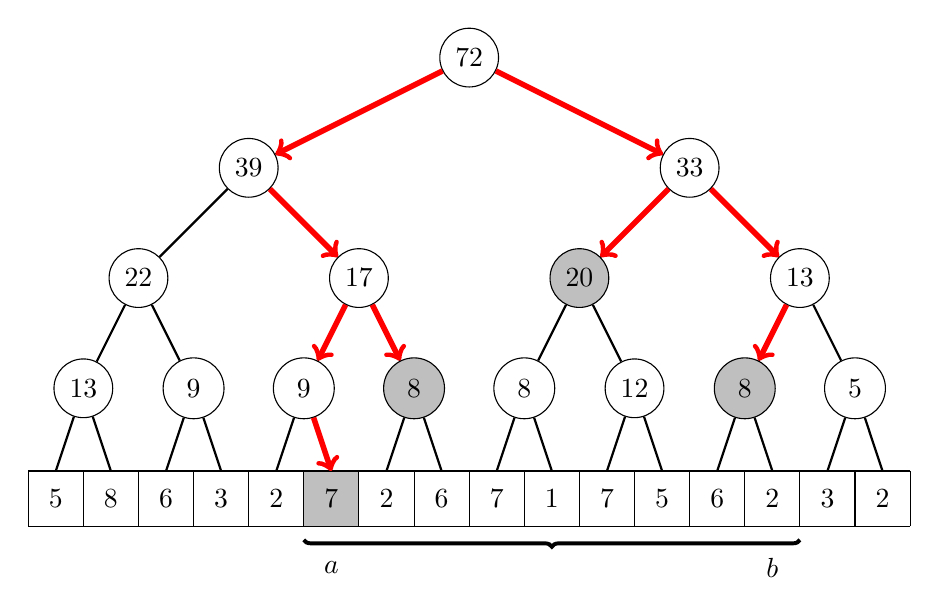
\begin{tikzpicture}[scale=0.7]
\fill[color=gray!50] (5,0) rectangle (6,1);
\draw (0,0) grid (16,1);

\node[anchor=center] at (0.5, 0.5) {5};
\node[anchor=center] at (1.5, 0.5) {8};
\node[anchor=center] at (2.5, 0.5) {6};
\node[anchor=center] at (3.5, 0.5) {3};
\node[anchor=center] at (4.5, 0.5) {2};
\node[anchor=center] at (5.5, 0.5) {7};
\node[anchor=center] at (6.5, 0.5) {2};
\node[anchor=center] at (7.5, 0.5) {6};
\node[anchor=center] at (8.5, 0.5) {7};
\node[anchor=center] at (9.5, 0.5) {1};
\node[anchor=center] at (10.5, 0.5) {7};
\node[anchor=center] at (11.5, 0.5) {5};
\node[anchor=center] at (12.5, 0.5) {6};
\node[anchor=center] at (13.5, 0.5) {2};
\node[anchor=center] at (14.5, 0.5) {3};
\node[anchor=center] at (15.5, 0.5) {2};

%\node[anchor=center] at (1,2.5) {13};

\node[draw, circle] (a) at (1,2.5) {13};
\path[draw,thick,-] (a) -- (0.5,1);
\path[draw,thick,-] (a) -- (1.5,1);
\node[draw, circle,minimum size=22pt] (b) at (3,2.5) {9};
\path[draw,thick,-] (b) -- (2.5,1);
\path[draw,thick,-] (b) -- (3.5,1);
\node[draw, circle,minimum size=22pt] (c) at (5,2.5) {9};
\path[draw,thick,-] (c) -- (4.5,1);
\path[draw,thick,-] (c) -- (5.5,1);
\node[draw, circle,fill=gray!50,minimum size=22pt] (d) at (7,2.5) {8};
\path[draw,thick,-] (d) -- (6.5,1);
\path[draw,thick,-] (d) -- (7.5,1);
\node[draw, circle,minimum size=22pt] (e) at (9,2.5) {8};
\path[draw,thick,-] (e) -- (8.5,1);
\path[draw,thick,-] (e) -- (9.5,1);
\node[draw, circle] (f) at (11,2.5) {12};
\path[draw,thick,-] (f) -- (10.5,1);
\path[draw,thick,-] (f) -- (11.5,1);
\node[draw, circle,fill=gray!50,minimum size=22pt] (g) at (13,2.5) {8};
\path[draw,thick,-] (g) -- (12.5,1);
\path[draw,thick,-] (g) -- (13.5,1);
\node[draw, circle,minimum size=22pt] (h) at (15,2.5) {5};
\path[draw,thick,-] (h) -- (14.5,1);
\path[draw,thick,-] (h) -- (15.5,1);

\node[draw, circle] (i) at (2,4.5) {22};
\path[draw,thick,-] (i) -- (a);
\path[draw,thick,-] (i) -- (b);
\node[draw, circle] (j) at (6,4.5) {17};
\path[draw,thick,-] (j) -- (c);
\path[draw,thick,-] (j) -- (d);
\node[draw, circle,fill=gray!50] (k) at (10,4.5) {20};
\path[draw,thick,-] (k) -- (e);
\path[draw,thick,-] (k) -- (f);
\node[draw, circle] (l) at (14,4.5) {13};
\path[draw,thick,-] (l) -- (g);
\path[draw,thick,-] (l) -- (h);

\node[draw, circle] (m) at (4,6.5) {39};
\path[draw,thick,-] (m) -- (i);
\path[draw,thick,-] (m) -- (j);
\node[draw, circle] (n) at (12,6.5) {33};
\path[draw,thick,-] (n) -- (k);
\path[draw,thick,-] (n) -- (l);

\node[draw, circle] (o) at (8,8.5) {72};
\path[draw,thick,-] (o) -- (m);
\path[draw,thick,-] (o) -- (n);

\path[draw=red,thick,->,line width=2pt] (o) -- (m);
\path[draw=red,thick,->,line width=2pt] (o) -- (n);

\path[draw=red,thick,->,line width=2pt] (m) -- (j);
\path[draw=red,thick,->,line width=2pt] (j) -- (c);
\path[draw=red,thick,->,line width=2pt] (j) -- (d);
\path[draw=red,thick,->,line width=2pt] (c) -- (5.5,1);

\path[draw=red,thick,->,line width=2pt] (n) -- (k);
\path[draw=red,thick,->,line width=2pt] (n) -- (l);

\path[draw=red,thick,->,line width=2pt] (l) -- (g);

\draw [decoration={brace}, decorate, line width=0.5mm] (14,-0.25) -- (5,-0.25);

\node at (5.5,-0.75) {$a$};
\node at (13.5,-0.75) {$b$};
\end{tikzpicture}
\end{center}

همچنین در این پیاده‌سازی،
عملیات‌ها به زمان $O(\log n)$ نیاز دارند،
زیرا تعداد کل رأس‌های دیده‌شده $O(\log n)$ است.

\section{انتشار تنبل}

\index{انتشار تنبل}
\index{درخت پاره‌خطی تنبل}

با استفاده از \key{انتشار تنبل} (lazy propagation)، می‌توان
درخت پاره‌خطی ساخت که \emph{هم} به‌روزرسانی‌های بازه‌ای
و \emph{هم} پرس‌وجوهای بازه‌ای را در زمان $O(\log n)$ پشتیبانی کند.
ایده کار، انجام به‌روزرسانی‌ها و پرس‌وجوها
از بالا به پایین و اجرای به‌روزرسانی‌ها به‌صورت
\emph{تنبل} است، به طوری که تنها در صورت نیاز
به سمت پایین درخت منتشر شوند.

در یک درخت بازه‌ای با انتشار تنبل (lazy segment tree)، گره‌ها حاوی دو نوع اطلاعات هستند.
مانند درخت بازه‌ای معمولی، هر گره شامل مجموع یا مقدار دیگری مرتبط با زیرآرایه متناظر است.
علاوه بر این، گره می‌تواند حاوی اطلاعات مربوط به به‌روزرسانی‌های تنبل باشد که هنوز به فرزندان آن منتقل نشده است.

دو نوع به‌روزرسانی بازه‌ای وجود دارد:
هر مقدار آرایه در بازه یا با مقداری \emph{افزایش} می‌یابد
یا مقداری به آن \emph{انتساب} داده می‌شود.
هر دو عملیات را می‌توان با ایده‌های مشابه پیاده‌سازی کرد و حتی ساخت درختی که هم‌زمان از هر دو عملیات پشتیبانی کند نیز ممکن است.

\subsubsection{درخت‌های بازه‌ای تنبل}

مثالی را در نظر بگیرید که در آن هدف ما ساخت یک درخت بازه‌ای است که از دو عملیات پشتیبانی کند:
افزایش هر مقدار در $[a,b]$ با یک مقدار ثابت و محاسبه مجموع مقادیر در $[a,b]$.

درختی می‌سازیم که هر گره آن دو مقدار $s/z$ دارد:
$s$ نشان‌دهنده مجموع مقادیر در بازه است
و $z$ مقدار به‌روزرسانی تنبل را نشان می‌دهد،
به این معنی که تمام مقادیر در بازه باید به اندازه $z$ افزایش یابند.
در درخت زیر، در تمام گره‌ها $z=0$ است،
بنابراین هیچ به‌روزرسانی تنبل در جریانی وجود ندارد.
\begin{center}
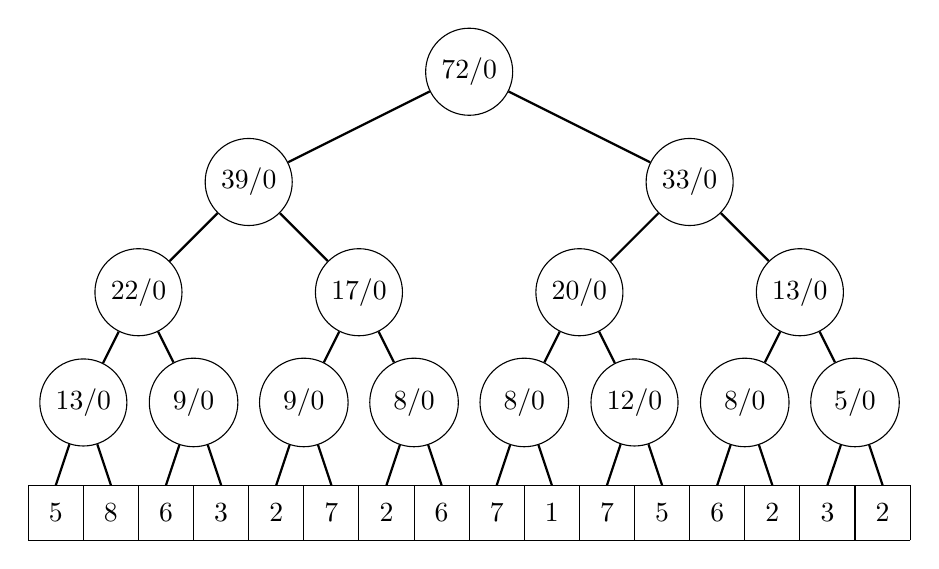
\begin{tikzpicture}[scale=0.7]
\draw (0,0) grid (16,1);

\node[anchor=center] at (0.5, 0.5) {5};
\node[anchor=center] at (1.5, 0.5) {8};
\node[anchor=center] at (2.5, 0.5) {6};
\node[anchor=center] at (3.5, 0.5) {3};
\node[anchor=center] at (4.5, 0.5) {2};
\node[anchor=center] at (5.5, 0.5) {7};
\node[anchor=center] at (6.5, 0.5) {2};
\node[anchor=center] at (7.5, 0.5) {6};
\node[anchor=center] at (8.5, 0.5) {7};
\node[anchor=center] at (9.5, 0.5) {1};
\node[anchor=center] at (10.5, 0.5) {7};
\node[anchor=center] at (11.5, 0.5) {5};
\node[anchor=center] at (12.5, 0.5) {6};
\node[anchor=center] at (13.5, 0.5) {2};
\node[anchor=center] at (14.5, 0.5) {3};
\node[anchor=center] at (15.5, 0.5) {2};

\node[draw, circle] (a) at (1,2.5) {13/0};
\path[draw,thick,-] (a) -- (0.5,1);
\path[draw,thick,-] (a) -- (1.5,1);
\node[draw, circle,minimum size=32pt] (b) at (3,2.5) {9/0};
\path[draw,thick,-] (b) -- (2.5,1);
\path[draw,thick,-] (b) -- (3.5,1);
\node[draw, circle,minimum size=32pt] (c) at (5,2.5) {9/0};
\path[draw,thick,-] (c) -- (4.5,1);
\path[draw,thick,-] (c) -- (5.5,1);
\node[draw, circle,minimum size=32pt] (d) at (7,2.5) {8/0};
\path[draw,thick,-] (d) -- (6.5,1);
\path[draw,thick,-] (d) -- (7.5,1);
\node[draw, circle,minimum size=32pt] (e) at (9,2.5) {8/0};
\path[draw,thick,-] (e) -- (8.5,1);
\path[draw,thick,-] (e) -- (9.5,1);
\node[draw, circle] (f) at (11,2.5) {12/0};
\path[draw,thick,-] (f) -- (10.5,1);
\path[draw,thick,-] (f) -- (11.5,1);
\node[draw, circle,minimum size=32pt] (g) at (13,2.5) {8/0};
\path[draw,thick,-] (g) -- (12.5,1);
\path[draw,thick,-] (g) -- (13.5,1);
\node[draw, circle,minimum size=32pt] (h) at (15,2.5) {5/0};
\path[draw,thick,-] (h) -- (14.5,1);
\path[draw,thick,-] (h) -- (15.5,1);

\node[draw, circle] (i) at (2,4.5) {22/0};
\path[draw,thick,-] (i) -- (a);
\path[draw,thick,-] (i) -- (b);
\node[draw, circle] (j) at (6,4.5) {17/0};
\path[draw,thick,-] (j) -- (c);
\path[draw,thick,-] (j) -- (d);
\node[draw, circle] (k) at (10,4.5) {20/0};
\path[draw,thick,-] (k) -- (e);
\path[draw,thick,-] (k) -- (f);
\node[draw, circle] (l) at (14,4.5) {13/0};
\path[draw,thick,-] (l) -- (g);
\path[draw,thick,-] (l) -- (h);

\node[draw, circle] (m) at (4,6.5) {39/0};
\path[draw,thick,-] (m) -- (i);
\path[draw,thick,-] (m) -- (j);
\node[draw, circle] (n) at (12,6.5) {33/0};
\path[draw,thick,-] (n) -- (k);
\path[draw,thick,-] (n) -- (l);

\node[draw, circle] (o) at (8,8.5) {72/0};
\path[draw,thick,-] (o) -- (m);
\path[draw,thick,-] (o) -- (n);
\end{tikzpicture}
\end{center}

وقتی مقادیر بازه $[a,b]$ به اندازه $u$ افزایش می‌یابند،
از ریشه به سمت برگ‌ها حرکت می‌کنیم
و گره‌های درخت را به این شکل تغییر می‌دهیم:
اگر بازه $[x,y]$ مربوط به یک گره
کاملاً درون $[a,b]$ قرار گیرد،
مقدار $z$ گره را $u$ واحد افزایش می‌دهیم و متوقف می‌شویم.
اگر $[x,y]$ تنها بخشی از $[a,b]$ را پوشش دهد،
مقدار $s$ گره را به اندازه $hu$ افزایش می‌دهیم؛
طوری که $h$ اندازه اشتراک $[a,b]$
و $[x,y]$ است، سپس پیمایش بازگشتی در درخت را ادامه می‌دهیم.

برای نمونه، تصویر زیر درخت را پس از
افزایش عناصر بازه $[a,b]$ به اندازه ۲ نشان می‌دهد:
\begin{center}
\begin{tikzpicture}[scale=0.7]
\fill[color=gray!50] (5,0) rectangle (6,1);
\draw (0,0) grid (16,1);

\node[anchor=center] at (0.5, 0.5) {5};
\node[anchor=center] at (1.5, 0.5) {8};
\node[anchor=center] at (2.5, 0.5) {6};
\node[anchor=center] at (3.5, 0.5) {3};
\node[anchor=center] at (4.5, 0.5) {2};
\node[anchor=center] at (5.5, 0.5) {9};
\node[anchor=center] at (6.5, 0.5) {2};
\node[anchor=center] at (7.5, 0.5) {6};
\node[anchor=center] at (8.5, 0.5) {7};
\node[anchor=center] at (9.5, 0.5) {1};
\node[anchor=center] at (10.5, 0.5) {7};
\node[anchor=center] at (11.5, 0.5) {5};
\node[anchor=center] at (12.5, 0.5) {6};
\node[anchor=center] at (13.5, 0.5) {2};
\node[anchor=center] at (14.5, 0.5) {3};
\node[anchor=center] at (15.5, 0.5) {2};

\node[draw, circle] (a) at (1,2.5) {13/0};
\path[draw,thick,-] (a) -- (0.5,1);
\path[draw,thick,-] (a) -- (1.5,1);
\node[draw, circle,minimum size=32pt] (b) at (3,2.5) {9/0};
\path[draw,thick,-] (b) -- (2.5,1);
\path[draw,thick,-] (b) -- (3.5,1);
\node[draw, circle,minimum size=32pt] (c) at (5,2.5) {11/0};
\path[draw,thick,-] (c) -- (4.5,1);
\path[draw,thick,-] (c) -- (5.5,1);
\node[draw, circle,fill=gray!50,minimum size=32pt] (d) at (7,2.5) {8/2};
\path[draw,thick,-] (d) -- (6.5,1);
\path[draw,thick,-] (d) -- (7.5,1);
\node[draw, circle,size=32pt] (e) at (9,2.5) {8/0};
\path[draw,thick,-] (e) -- (8.5,1);
\path[draw,thick,-] (e) -- (9.5,1);
\node[draw, circle] (f) at (11,2.5) {12/0};
\path[draw,thick,-] (f) -- (10.5,1);
\path[draw,thick,-] (f) -- (11.5,1);
\node[draw, circle,fill=gray!50,minimum size=32pt] (g) at (13,2.5) {8/2};
\path[draw,thick,-] (g) -- (12.5,1);
\path[draw,thick,-] (g) -- (13.5,1);
\node[draw, circle,minimum size=32pt] (h) at (15,2.5) {5/0};
\path[draw,thick,-] (h) -- (14.5,1);
\path[draw,thick,-] (h) -- (15.5,1);

\node[draw, circle] (i) at (2,4.5) {22/0};
\path[draw,thick,-] (i) -- (a);
\path[draw,thick,-] (i) -- (b);
\node[draw, circle] (j) at (6,4.5) {23/0};
\path[draw,thick,-] (j) -- (c);
\path[draw,thick,-] (j) -- (d);
\node[draw, circle,fill=gray!50] (k) at (10,4.5) {20/2};
\path[draw,thick,-] (k) -- (e);
\path[draw,thick,-] (k) -- (f);
\node[draw, circle] (l) at (14,4.5) {17/0};
\path[draw,thick,-] (l) -- (g);
\path[draw,thick,-] (l) -- (h);

\node[draw, circle] (m) at (4,6.5) {45/0};
\path[draw,thick,-] (m) -- (i);
\path[draw,thick,-] (m) -- (j);
\node[draw, circle] (n) at (12,6.5) {45/0};
\path[draw,thick,-] (n) -- (k);
\path[draw,thick,-] (n) -- (l);

\node[draw, circle] (o) at (8,8.5) {90/0};
\path[draw,thick,-] (o) -- (m);
\path[draw,thick,-] (o) -- (n);

\path[draw=red,thick,->,line width=2pt] (o) -- (m);
\path[draw=red,thick,->,line width=2pt] (o) -- (n);

\path[draw=red,thick,->,line width=2pt] (m) -- (j);
\path[draw=red,thick,->,line width=2pt] (j) -- (c);
\path[draw=red,thick,->,line width=2pt] (j) -- (d);
\path[draw=red,thick,->,line width=2pt] (c) -- (5.5,1);

\path[draw=red,thick,->,line width=2pt] (n) -- (k);
\path[draw=red,thick,->,line width=2pt] (n) -- (l);

\path[draw=red,thick,->,line width=2pt] (l) -- (g);

\draw [decoration={brace}, decorate, line width=0.5mm] (14,-0.25) -- (5,-0.25);

\node at (5.5,-0.75) {$a$};
\node at (13.5,-0.75) {$b$};
\end{tikzpicture}
\end{center}

همچنین مجموع عناصر در بازه $[a,b]$ را با پیمایش درخت از بالا به پایین محاسبه می‌کنیم.
اگر بازه $[x,y]$ مربوط به یک گره به‌طور کامل درون $[a,b]$ قرار گیرد، مقدار $s$ آن گره را به مجموع اضافه می‌کنیم.
در غیر این صورت، جستجو را به‌صورت بازگشتی به سمت پایین درخت ادامه می‌دهیم.

هم در به‌روزرسانی‌ها و هم در پرس‌وجوها،
مقدار به‌روزرسانی تنبل همیشه قبل از پردازش گره
به فرزندان آن منتقل می‌شود.
ایده این است که به‌روزرسانی‌ها فقط در صورت نیاز
به سمت پایین منتشر شوند،
که کارآمد بودن همیشگی عملیات‌ها را تضمین می‌کند.

تصویر زیر تغییرات درخت را هنگام محاسبه مقدار $\texttt{sum}_a(a,b)$ نشان می‌دهد.
مستطیل گره‌هایی را نشان می‌دهد که مقادیر آن‌ها به دلیل انتشار به‌روزرسانی تنبل به سمت پایین تغییر می‌کند.

\begin{center}
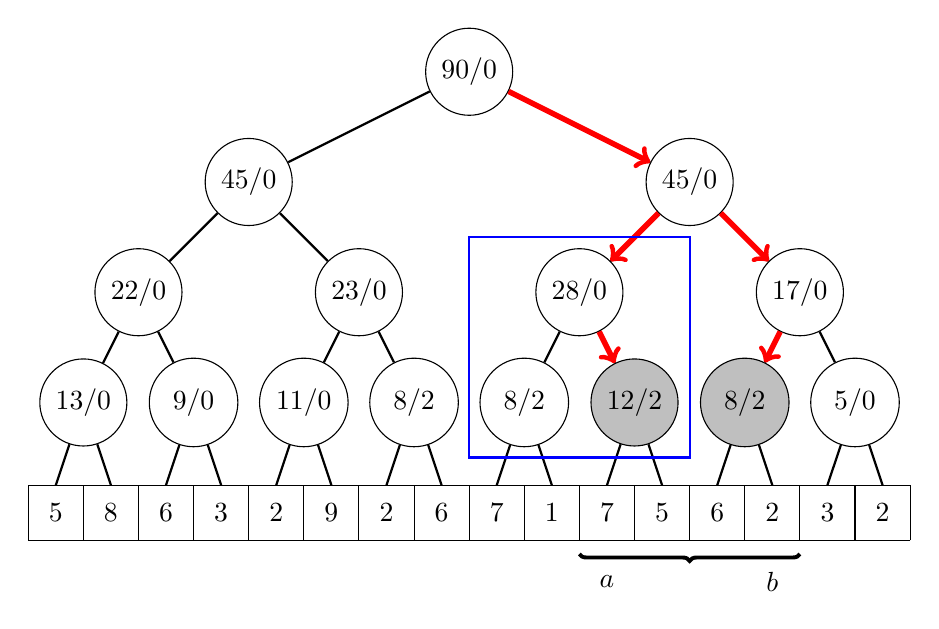
\begin{tikzpicture}[scale=0.7]
\draw (0,0) grid (16,1);

\node[anchor=center] at (0.5, 0.5) {5};
\node[anchor=center] at (1.5, 0.5) {8};
\node[anchor=center] at (2.5, 0.5) {6};
\node[anchor=center] at (3.5, 0.5) {3};
\node[anchor=center] at (4.5, 0.5) {2};
\node[anchor=center] at (5.5, 0.5) {9};
\node[anchor=center] at (6.5, 0.5) {2};
\node[anchor=center] at (7.5, 0.5) {6};
\node[anchor=center] at (8.5, 0.5) {7};
\node[anchor=center] at (9.5, 0.5) {1};
\node[anchor=center] at (10.5, 0.5) {7};
\node[anchor=center] at (11.5, 0.5) {5};
\node[anchor=center] at (12.5, 0.5) {6};
\node[anchor=center] at (13.5, 0.5) {2};
\node[anchor=center] at (14.5, 0.5) {3};
\node[anchor=center] at (15.5, 0.5) {2};

\node[draw, circle] (a) at (1,2.5) {13/0};
\path[draw,thick,-] (a) -- (0.5,1);
\path[draw,thick,-] (a) -- (1.5,1);
\node[draw, circle,minimum size=32pt] (b) at (3,2.5) {9/0};
\path[draw,thick,-] (b) -- (2.5,1);
\path[draw,thick,-] (b) -- (3.5,1);
\node[draw, circle,minimum size=32pt] (c) at (5,2.5) {11/0};
\path[draw,thick,-] (c) -- (4.5,1);
\path[draw,thick,-] (c) -- (5.5,1);
\node[draw, circle,minimum size=32pt] (d) at (7,2.5) {8/2};
\path[draw,thick,-] (d) -- (6.5,1);
\path[draw,thick,-] (d) -- (7.5,1);
\node[draw, circle,minimum size=32pt] (e) at (9,2.5) {8/2};
\path[draw,thick,-] (e) -- (8.5,1);
\path[draw,thick,-] (e) -- (9.5,1);
\node[draw, circle,fill=gray!50,] (f) at (11,2.5) {12/2};
\path[draw,thick,-] (f) -- (10.5,1);
\path[draw,thick,-] (f) -- (11.5,1);
\node[draw, circle,fill=gray!50,minimum size=32pt] (g) at (13,2.5) {8/2};
\path[draw,thick,-] (g) -- (12.5,1);
\path[draw,thick,-] (g) -- (13.5,1);
\node[draw, circle,minimum size=32pt] (h) at (15,2.5) {5/0};
\path[draw,thick,-] (h) -- (14.5,1);
\path[draw,thick,-] (h) -- (15.5,1);

\node[draw, circle] (i) at (2,4.5) {22/0};
\path[draw,thick,-] (i) -- (a);
\path[draw,thick,-] (i) -- (b);
\node[draw, circle] (j) at (6,4.5) {23/0};
\path[draw,thick,-] (j) -- (c);
\path[draw,thick,-] (j) -- (d);
\node[draw, circle] (k) at (10,4.5) {28/0};
\path[draw,thick,-] (k) -- (e);
\path[draw,thick,-] (k) -- (f);
\node[draw, circle] (l) at (14,4.5) {17/0};
\path[draw,thick,-] (l) -- (g);
\path[draw,thick,-] (l) -- (h);

\node[draw, circle] (m) at (4,6.5) {45/0};
\path[draw,thick,-] (m) -- (i);
\path[draw,thick,-] (m) -- (j);
\node[draw, circle] (n) at (12,6.5) {45/0};
\path[draw,thick,-] (n) -- (k);
\path[draw,thick,-] (n) -- (l);

\node[draw, circle] (o) at (8,8.5) {90/0};
\path[draw,thick,-] (o) -- (m);
\path[draw,thick,-] (o) -- (n);

\path[draw=red,thick,->,line width=2pt] (o) -- (n);

\path[draw=red,thick,->,line width=2pt] (n) -- (k);
\path[draw=red,thick,->,line width=2pt] (n) -- (l);

\path[draw=red,thick,->,line width=2pt] (k) -- (f);
\path[draw=red,thick,->,line width=2pt] (l) -- (g);

\draw [decoration={brace}, decorate, line width=0.5mm] (14,-0.25) -- (10,-0.25);

\draw[color=blue,thick] (8,1.5) rectangle (12,5.5);

\node at (10.5,-0.75) {$a$};
\node at (13.5,-0.75) {$b$};
\end{tikzpicture}
\end{center}

توجه کنید گاهی ترکیب به‌روزرسانی‌های تنبل نیاز است.
این حالت وقتی رخ می‌دهد که به گره دارای به‌روزرسانی تنبل، به‌روزرسانی تنبل دیگری تخصیص یابد.
هنگام محاسبه مجموع‌ها، ترکیب به‌روزرسانی‌های تنبل آسان است، زیرا ترکیب به‌روزرسانی‌های $z_1$ و $z_2$ معادل به‌روزرسانی $z_1+z_2$ است.

\subsubsection{به‌روزرسانی‌های چندجمله‌ای}

به‌روزرسانی‌های تنبل را می‌توان تعمیم داد تا امکان به‌روزرسانی بازه‌ها با چندجمله‌ای‌هایی به شکل زیر فراهم شود:
\[p(u) = t_k u^k + t_{k-1} u^{k-1} + \cdots + t_0.\]

در این حالت، مقدار به‌روزرسانی برای خانه در موقعیت $i$ در بازه $[a,b]$ برابر با $p(i-a)$ است.
برای نمونه، افزودن چندجمله‌ای $p(u)=u+1$ به $[a,b]$ یعنی مقدار موقعیت $a$ به اندازه ۱، مقدار موقعیت $a+1$ به اندازه ۲ و به همین ترتیب افزایش می‌یابد.

برای پشتیبانی از به‌روزرسانی‌های چندجمله‌ای، به هر گره $k+2$ مقدار تخصیص می‌یابد که در آن $k$ برابر درجه چندجمله‌ای است.
مقدار $s$ مجموع عناصر بازه است، و مقادیر $z_0,z_1,\ldots,z_k$ ضرایب چندجمله‌ای متناظر با به‌روزرسانی تنبل هستند.

اکنون مجموع مقادیر در بازه $[x,y]$ برابر است با:
\[s+\sum_{u=0}^{y-x} z_k u^k + z_{k-1} u^{k-1} + \cdots + z_0.\]

مقدار این مجموع را می‌توان با فرمول‌های مجموع با کارایی بالا محاسبه کرد.
برای نمونه، جمله $z_0$ متناظر با مجموع $(y-x+1)z_0$ است، و جمله $z_1 u$ متناظر است با مجموع:
\[z_1(0+1+\cdots+y-x) = z_1 \frac{(y-x)(y-x+1)}{2} .\]

هنگام انتشار به‌روزرسانی در درخت، اندیس‌های $p(u)$ تغییر می‌کنند، زیرا در هر بازه $[x,y]$ مقادیر برای $u=0,1,\ldots,y-x$ محاسبه می‌شوند.
با این حال مشکلی نیست، زیرا $p'(u)=p(u+h)$ چندجمله‌ای با درجه برابر با $p(u)$ است.
برای نمونه اگر $p(u)=t_2 u^2+t_1 u-t_0$ باشد، آنگاه:
\[p'(u)=t_2(u+h)^2+t_1(u+h)-t_0=t_2 u^2 + (2ht_2+t_1)u+t_2h^2+t_1h-t_0.\]

\section{درخت‌های پویا}

\index{درخت پاره‌خطی پویا}

درخت پاره‌خطی معمولی ایستا است؛ یعنی هر گره جایگاه ثابتی در آرایه دارد و درخت به مقدار ثابتی حافظه نیاز دارد.
در \key{درخت پاره‌خطی پویا}، حافظه تنها به گره‌هایی تخصیص می‌یابد که در طول اجرای الگوریتم واقعاً پیمایش می‌شوند؛ این کار صرفه‌جویی بالایی در حافظه ایجاد می‌کند.

گره‌های یک درخت پویا می‌توانند به صورت ساختار (struct) پیاده‌سازی شوند:
\begin{lstlisting}
struct node {
    int value;
    int x, y;
    node *left, *right;
    node(int v, int x, int y) : value(v), x(x), y(y) {}
};
\end{lstlisting}
در اینجا \texttt{value} مقدار گره است،
$[\texttt{x},\texttt{y}]$ بازه متناظر است،
و \texttt{left} و \texttt{right} به زیردرخت چپ
و راست اشاره می‌کنند.

پس از این، گره‌ها می‌توانند به صورت زیر ایجاد شوند:
\begin{lstlisting}
// create new node
node *x = new node(0, 0, 15);
// change value
x->value = 5;
\end{lstlisting}

\subsubsection{درخت‌های بخش‌بندی تنک}

\index{sparse segment tree}

یک درخت بخش‌بندی پویا زمانی مفید است که
آرایه زیرین \emph{تنک} (sparse) باشد؛
به این معنی که بازه $[0,n-1]$ از اندیس‌های مجاز بزرگ است،
اما بیشتر مقادیر آرایه صفر هستند.
در حالی که یک درخت بخش‌بندی معمولی از $O(n)$ حافظه استفاده می‌کند،
یک درخت بخش‌بندی پویا تنها از $O(k \log n)$ حافظه مصرف می‌نماید،
که در آن $k$ تعداد عملیات‌های انجام‌شده است.

یک \key{درخت بخش‌بندی تنک} در ابتدا تنها
یک گره $[0,n-1]$ دارد که مقدار آن صفر است؛
بدین معنا که هر مقدار آرایه برابر صفر است.
پس از به‌روزرسانی‌ها، گره‌های جدید به صورت پویا
به درخت اضافه می‌شوند.
برای مثال، اگر $n=16$ باشد و عناصر
موقعیت‌های 3 و 10 تغییر یافته باشند،
درخت شامل گره‌های زیر خواهد بود:
\begin{center}
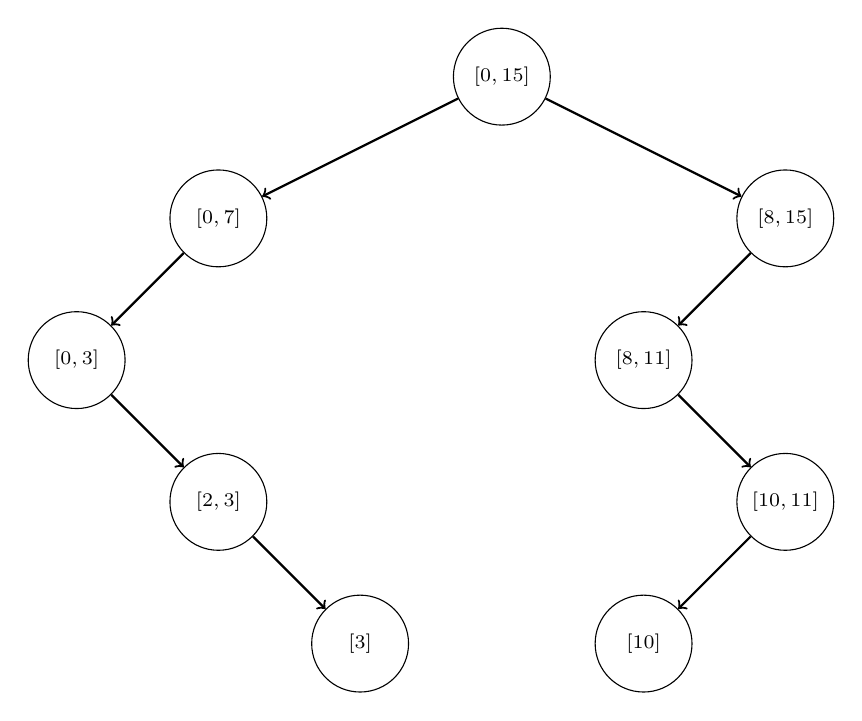
\begin{tikzpicture}[scale=0.9]
\scriptsize
\node[draw, circle,minimum size=35pt] (1) at (0,0) {$[0,15]$};
\node[draw, circle,minimum size=35pt] (2) at (-4,-2) {$[0,7]$};
\node[draw, circle,minimum size=35pt] (3) at (-6,-4) {$[0,3]$};
\node[draw, circle,minimum size=35pt] (4) at (-4,-6) {$[2,3]$};
\node[draw, circle,minimum size=35pt] (5) at (-2,-8) {$[3]$};
\node[draw, circle,minimum size=35pt] (6) at (4,-2) {$[8,15]$};
\node[draw, circle,minimum size=35pt] (7) at (2,-4) {$[8,11]$};
\node[draw, circle,minimum size=35pt] (8) at (4,-6) {$[10,11]$};
\node[draw, circle,minimum size=35pt] (9) at (2,-8) {$[10]$};

\path[draw,thick,->] (1) -- (2);
\path[draw,thick,->] (2) -- (3);
\path[draw,thick,->] (3) -- (4);
\path[draw,thick,->] (4) -- (5);

\path[draw,thick,->] (1) -- (6);
\path[draw,thick,->] (6) -- (7);
\path[draw,thick,->] (7) -- (8);
\path[draw,thick,->] (8) -- (9);
\end{tikzpicture}
\end{center}

هر مسیر از گره ریشه تا یک برگ شامل
$O(\log n)$ گره است،
بنابراین هر عملیات حداکثر $O(\log n)$
گره جدید به درخت اضافه می‌کند.
از این رو، پس از $k$ عملیات، درخت شامل
حداکثر $O(k \log n)$ گره خواهد بود.

توجه داشته باشید اگر تمام عناصری را که باید به‌روزرسانی شوند
در آغاز الگوریتم بدانیم،
نیازی به درخت بخش‌بندی پویا نیست،
زیرا می‌توانیم از یک درخت بخش‌بندی معمولی همراه با
فشرده‌سازی مختصات (فصل 9.4) استفاده کنیم.
با این حال، زمانی که اندیس‌ها در طول اجرای الگوریتم تولید می‌شوند،
این کار امکان‌پذیر نیست.

\subsubsection{درخت‌های بخش‌بندی پایدار}

\index{persistent segment tree}

با استفاده از پیاده‌سازی پویا،
ساخت \key{درخت بازه‌ای پایا} (persistent segment tree)
نیز ممکن است که \emph{تاریخچه تغییرات} درخت را ذخیره می‌کند.
در این پیاده‌سازی، دسترسی کارآمد به تمام نسخه‌های موجود درخت
در طول الگوریتم امکان‌پذیر است.

هنگام در دسترس بودن تاریخچه تغییرات،
اجرای پرس‌وجوها روی هر نسخه پیشین مانند درخت بازه‌ای معمولی انجام می‌شود،
زیرا ساختار کامل هر درخت ذخیره شده است.
همچنین ساخت درخت‌های جدید بر پایه درخت‌های پیشین و تغییر مستقل آن‌ها ممکن است.

توالی به‌روزرسانی‌های زیر را در نظر بگیرید
که در آن گره‌های قرمز تغییر می‌کنند
و سایر گره‌ها ثابت می‌مانند:

\begin{center}
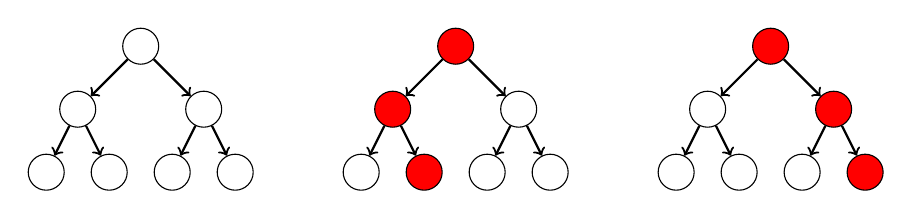
\begin{tikzpicture}[scale=0.8]
\node[draw, circle,minimum size=13pt] (1a) at (3,0) {};
\node[draw, circle,minimum size=13pt] (2a) at (2,-1) {};
\node[draw, circle,minimum size=13pt] (3a) at (4,-1) {};
\node[draw, circle,minimum size=13pt] (4a) at (1.5,-2) {};
\node[draw, circle,minimum size=13pt] (5a) at (2.5,-2) {};
\node[draw, circle,minimum size=13pt] (6a) at (3.5,-2) {};
\node[draw, circle,minimum size=13pt] (7a) at (4.5,-2) {};
\path[draw,thick,->] (1a) -- (2a);
\path[draw,thick,->] (1a) -- (3a);
\path[draw,thick,->] (2a) -- (4a);
\path[draw,thick,->] (2a) -- (5a);
\path[draw,thick,->] (3a) -- (6a);
\path[draw,thick,->] (3a) -- (7a);

\node[draw, circle,minimum size=13pt,fill=red] (1b) at (3+5,0) {};
\node[draw, circle,minimum size=13pt,fill=red] (2b) at (2+5,-1) {};
\node[draw, circle,minimum size=13pt] (3b) at (4+5,-1) {};
\node[draw, circle,minimum size=13pt] (4b) at (1.5+5,-2) {};
\node[draw, circle,minimum size=13pt,fill=red] (5b) at (2.5+5,-2) {};
\node[draw, circle,minimum size=13pt] (6b) at (3.5+5,-2) {};
\node[draw, circle,minimum size=13pt] (7b) at (4.5+5,-2) {};
\path[draw,thick,->] (1b) -- (2b);
\path[draw,thick,->] (1b) -- (3b);
\path[draw,thick,->] (2b) -- (4b);
\path[draw,thick,->] (2b) -- (5b);
\path[draw,thick,->] (3b) -- (6b);
\path[draw,thick,->] (3b) -- (7b);

\node[draw, circle,minimum size=13pt,fill=red] (1c) at (3+10,0) {};
\node[draw, circle,minimum size=13pt] (2c) at (2+10,-1) {};
\node[draw, circle,minimum size=13pt,fill=red] (3c) at (4+10,-1) {};
\node[draw, circle,minimum size=13pt] (4c) at (1.5+10,-2) {};
\node[draw, circle,minimum size=13pt] (5c) at (2.5+10,-2) {};
\node[draw, circle,minimum size=13pt] (6c) at (3.5+10,-2) {};
\node[draw, circle,minimum size=13pt,fill=red] (7c) at (4.5+10,-2) {};
\path[draw,thick,->] (1c) -- (2c);
\path[draw,thick,->] (1c) -- (3c);
\path[draw,thick,->] (2c) -- (4c);
\path[draw,thick,->] (2c) -- (5c);
\path[draw,thick,->] (3c) -- (6c);
\path[draw,thick,->] (3c) -- (7c);
\end{tikzpicture}
\end{center}

\node at (3,-3) {گام ۱};
\node at (3+5,-3) {گام ۲};
\node at (3+10,-3) {گام ۳};
\end{tikzpicture}
\end{center}
پس از هر به‌روزرسانی، بیشتر گره‌های درخت
دست‌نخورده باقی می‌مانند،
بنابراین روشی کارآمد برای ذخیرهٔ تاریخچهٔ تغییرات،
نمایش هر درخت در تاریخچه به‌صورت ترکیبی
از گره‌های جدید و زیردرخت‌های درختان قبلی است.
در این مثال، تاریخچهٔ تغییرات را می‌توان
به صورت زیر ذخیره کرد:
\begin{center}
\begin{tikzpicture}[scale=0.8]
\path[use as bounding box] (0, 1) rectangle (16, -3.5);

\node[draw, circle,minimum size=13pt] (1a) at (3,0) {};
\node[draw, circle,minimum size=13pt] (2a) at (2,-1) {};
\node[draw, circle,minimum size=13pt] (3a) at (4,-1) {};
\node[draw, circle,minimum size=13pt] (4a) at (1.5,-2) {};
\node[draw, circle,minimum size=13pt] (5a) at (2.5,-2) {};
\node[draw, circle,minimum size=13pt] (6a) at (3.5,-2) {};
\node[draw, circle,minimum size=13pt] (7a) at (4.5,-2) {};
\path[draw,thick,->] (1a) -- (2a);
\path[draw,thick,->] (1a) -- (3a);
\path[draw,thick,->] (2a) -- (4a);
\path[draw,thick,->] (2a) -- (5a);
\path[draw,thick,->] (3a) -- (6a);
\path[draw,thick,->] (3a) -- (7a);

\node[draw, circle,minimum size=13pt,fill=red] (1b) at (3+5,0) {};
\node[draw, circle,minimum size=13pt,fill=red] (2b) at (2+5,-1) {};
\node[draw, circle,minimum size=13pt,fill=red] (5b) at (2.5+5,-2) {};
\path[draw,thick,->] (1b) -- (2b);

\draw[thick,->] (1b) .. controls (3+5+2,0-1) and (3+5,2.5) .. (3a);

\draw[thick,->] (2b) .. controls (2+5-0.5,-1-0.5) and (2,4.5) .. (4a);


\path[draw,thick,->] (2b) -- (5b);

\node[draw, circle,minimum size=13pt,fill=red] (1c) at (3+10,0) {};
\node[draw, circle,minimum size=13pt,fill=red] (3c) at (4+10,-1) {};
\node[draw, circle,minimum size=13pt,fill=red] (7c) at (4.5+10,-2) {};
\path[draw,thick,->] (1c) -- (2b);
\path[draw,thick,->] (1c) -- (3c);

\draw[thick,->] (3c) .. controls (2.5+5,-3) and (3.5,-3) .. (6a);

\path[draw,thick,->] (3c) -- (7c);

\node at (3,-3) {گام ۱};
\node at (3+5,-3) {گام ۲};
\node at (3+10,-3) {گام ۳};
\end{tikzpicture}
\end{center}

ساختار هر درخت قبلی را می‌توان
با دنبال کردن اشاره‌گرها از گره ریشهٔ مربوطه
بازسازی کرد.
از آنجا که هر عملیات
تنها $O(\log n)$ گره جدید به درخت اضافه می‌کند،
ذخیرهٔ کل تاریخچهٔ تغییرات درخت ممکن است.

\section{ساختمان داده‌ها}

به جای مقادیر تکی، گره‌ها در درخت بازه‌ای
می‌توانند شامل \emph{ساختمان داده‌هایی} باشند که اطلاعات
مربوط به بازه‌ها را نگهداری می‌کنند.
در چنین درختی، عملیات‌ها به زمان
$O(f(n) \log n)$ نیاز دارند، که در آن $f(n)$
زمان مورد نیاز برای پردازش یک گره در حین عملیات است.

به عنوان مثال، درخت بازه‌ای را در نظر بگیرید که
پرسش‌هایی از این نوع را پشتیبانی می‌کند:
«عنصر $x$ چند بار
در بازهٔ $[a,b]$ تکرار شده است؟»
برای نمونه، عنصر ۱ سه بار
در بازهٔ زیر آمده است:

\begin{center}
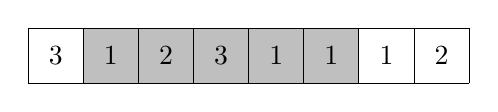
\begin{tikzpicture}[scale=0.7]
\fill[lightgray] (1,0) rectangle (6,1);
\draw (0,0) grid (8,1);

\node[anchor=center] at (0.5, 0.5) {3};
\node[anchor=center] at (1.5, 0.5) {1};
\node[anchor=center] at (2.5, 0.5) {2};
\node[anchor=center] at (3.5, 0.5) {3};
\node[anchor=center] at (4.5, 0.5) {1};
\node[anchor=center] at (5.5, 0.5) {1};
\node[anchor=center] at (6.5, 0.5) {1};
\node[anchor=center] at (7.5, 0.5) {2};
\end{tikzpicture}
\end{center}

برای پشتیبانی از چنین پرس‌وجوهایی، یک درخت بازه‌ای می‌سازیم
که به هر گره آن، ساختار داده‌ای اختصاص داده می‌شود
که می‌تواند تعداد دفعات تکرار هر عنصر دلخواه $x$
در بازه متناظر را پاسخ دهد.
با استفاده از این درخت،
پاسخ یک پرس‌وجو را می‌توان
از ترکیب نتایج گره‌های متعلق به بازه
محاسبه کرد.

برای مثال، درخت بازه‌ای زیر
متناظر با آرایه بالاست:
\begin{center}
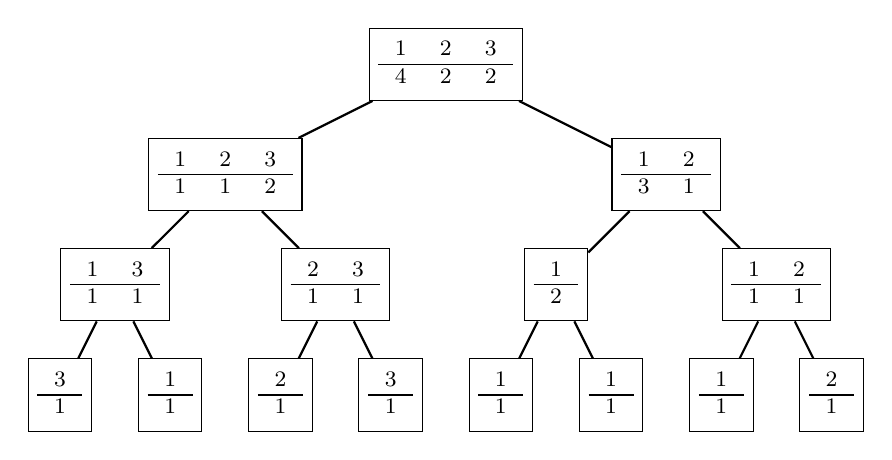
\begin{tikzpicture}[scale=0.7]

\node[draw, rectangle] (a) at (1,2.5)
{
\footnotesize
\begin{tabular}{r}
3 \\
\hline
1 \\
\end{tabular}};
\node[draw, rectangle] (b) at (3,2.5)
{
\footnotesize
\begin{tabular}{r}
1 \\
\hline
1 \\
\end{tabular}};
\node[draw, rectangle] (c) at (5,2.5)
{
\footnotesize
\begin{tabular}{r}
2 \\
\hline
1 \\
\end{tabular}};
\node[draw, rectangle] (d) at (7,2.5)
{
\footnotesize
\begin{tabular}{r}
3 \\
\hline
1 \\
\end{tabular}};
\node[draw, rectangle] (e) at (9,2.5)
{
\footnotesize
\begin{tabular}{r}
1 \\
\hline
1 \\
\end{tabular}};
\node[draw, rectangle] (f) at (11,2.5)
{
\footnotesize
\begin{tabular}{r}
1 \\
\hline
1 \\
\end{tabular}};
\node[draw, rectangle] (g) at (13,2.5)
{
\footnotesize
\begin{tabular}{r}
1 \\
\hline
1 \\
\end{tabular}};
\node[draw, rectangle] (h) at (15,2.5)
{
\footnotesize
\begin{tabular}{r}
2 \\
\hline
1 \\
\end{tabular}};

\node[draw, rectangle] (i) at (2,4.5)
{
\footnotesize
\begin{tabular}{rr}
1 & 3 \\
\hline
1 & 1 \\
\end{tabular}};
\path[draw,thick,-] (i) -- (a);
\path[draw,thick,-] (i) -- (b);
\node[draw, rectangle] (j) at (6,4.5)
{
\footnotesize
\begin{tabular}{rr}
2 & 3 \\
\hline
1 & 1 \\
\end{tabular}};
\path[draw,thick,-] (j) -- (c);
\path[draw,thick,-] (j) -- (d);
\node[draw, rectangle] (k) at (10,4.5)
{
\footnotesize
\begin{tabular}{r}
1 \\
\hline
2 \\
\end{tabular}};
\path[draw,thick,-] (k) -- (e);
\path[draw,thick,-] (k) -- (f);
\node[draw, rectangle] (l) at (14,4.5)
{
\footnotesize
\begin{tabular}{rr}
1 & 2 \\
\hline
1 & 1 \\
\end{tabular}};
\path[draw,thick,-] (l) -- (g);
\path[draw,thick,-] (l) -- (h);

\node[draw, rectangle] (m) at (4,6.5)
{
\footnotesize
\begin{tabular}{rrr}
1 & 2 & 3 \\
\hline
1 & 1 & 2 \\
\end{tabular}};
\path[draw,thick,-] (m) -- (i);
\path[draw,thick,-] (m) -- (j);
\node[draw, rectangle] (n) at (12,6.5)
{
\footnotesize
\begin{tabular}{rr}
1 & 2 \\
\hline
3 & 1 \\
\end{tabular}};
\path[draw,thick,-] (n) -- (k);
\path[draw,thick,-] (n) -- (l);

\node[draw, rectangle] (o) at (8,8.5)
{
\footnotesize
\begin{tabular}{rrr}
1 & 2 & 3 \\
\hline
4 & 2 & 2 \\
\end{tabular}};
\path[draw,thick,-] (o) -- (m);
\path[draw,thick,-] (o) -- (n);
\end{tikzpicture}
\end{center}

می‌توان درخت را طوری ساخت که هر رأس حاوی ساختار \texttt{map} باشد. در این حالت، زمان پردازش هر رأس $O(\log n)$ است؛ بنابراین پیچیدگی زمانی کل یک پرس‌وجو $O(\log^2 n)$ می‌شود. این درخت $O(n \log n)$ حافظه مصرف می‌کند، زیرا دارای $O(\log n)$ سطح است و هر سطح $O(n)$ عنصر دارد.

\section{حالت دوبعدی}

\index{two-dimensional segment tree}

یک \key{درخت پاره‌خطی دوبعدی} از پرس‌وجوهای مربوط به زیرآرایه‌های مستطیلی یک آرایه دوبعدی پشتیبانی می‌کند. چنین درختی می‌تواند به صورت درخت‌های پاره‌خطی تو در تو پیاده‌سازی شود: یک درخت بزرگ مربوط به سطرهای آرایه است، و هر رأس شامل یک درخت کوچک متناظر با ستون‌ها است.

برای مثال، در آرایه
\begin{center}
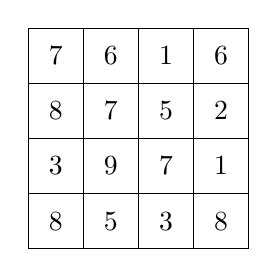
\begin{tikzpicture}[scale=0.7]
\draw (0,0) grid (4,4);

\node[anchor=center] at (0.5, 0.5) {8};
\node[anchor=center] at (1.5, 0.5) {5};
\node[anchor=center] at (2.5, 0.5) {3};
\node[anchor=center] at (3.5, 0.5) {8};

\node[anchor=center] at (0.5, 1.5) {3};
\node[anchor=center] at (1.5, 1.5) {9};
\node[anchor=center] at (2.5, 1.5) {7};
\node[anchor=center] at (3.5, 1.5) {1};

\node[anchor=center] at (0.5, 2.5) {8};
\node[anchor=center] at (1.5, 2.5) {7};
\node[anchor=center] at (2.5, 2.5) {5};
\node[anchor=center] at (3.5, 2.5) {2};

\node[anchor=center] at (0.5, 3.5) {7};
\node[anchor=center] at (1.5, 3.5) {6};
\node[anchor=center] at (2.5, 3.5) {1};
\node[anchor=center] at (3.5, 3.5) {6};
\end{tikzpicture}
\end{center}
مجموع هر زیرآرایه می‌تواند از درخت پاره‌خطی زیر محاسبه شود:
\begin{center}
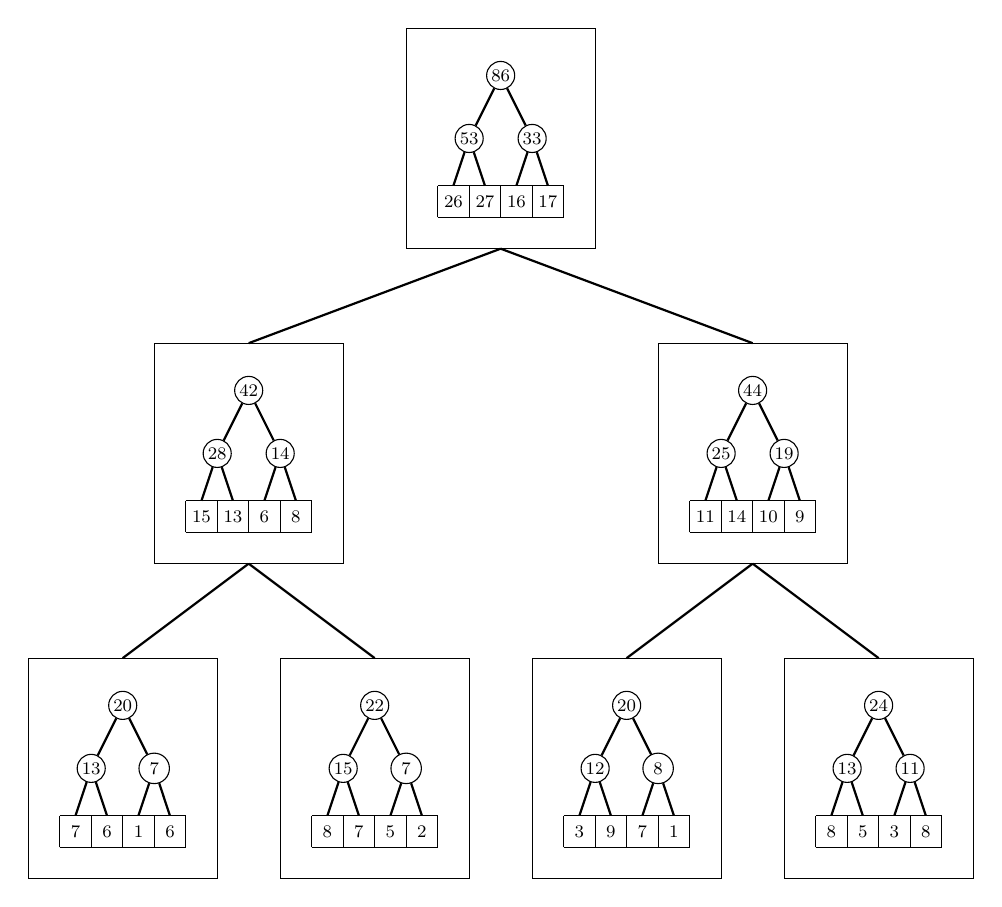
\begin{tikzpicture}[scale=0.4]
\footnotesize
\begin{scope}[shift={(-12,0)}]
\draw (-1,-1) rectangle (5,6);
\draw (0,0) grid (4,1);
\node[anchor=center,scale=0.8] at (0.5, 0.5) {7};
\node[anchor=center,scale=0.8] at (1.5, 0.5) {6};
\node[anchor=center,scale=0.8] at (2.5, 0.5) {1};
\node[anchor=center,scale=0.8] at (3.5, 0.5) {6};

\node[draw, circle,scale=0.8,inner sep=1pt] (a) at (1,2.5) {13};
\path[draw,thick,-] (a) -- (0.5,1);
\path[draw,thick,-] (a) -- (1.5,1);
\node[draw, circle,scale=0.8,inner sep=2.5pt] (b) at (3,2.5) {7};
\path[draw,thick,-] (b) -- (2.5,1);
\path[draw,thick,-] (b) -- (3.5,1);

\node[draw, circle,scale=0.8,inner sep=1pt] (i) at (2,4.5) {20};
\path[draw,thick,-] (i) -- (a);
\path[draw,thick,-] (i) -- (b);
\end{scope}
\begin{scope}[shift={(-4,0)}]
\draw (-1,-1) rectangle (5,6);
\draw (0,0) grid (4,1);
\node[anchor=center,scale=0.8] at (0.5, 0.5) {8};
\node[anchor=center,scale=0.8] at (1.5, 0.5) {7};
\node[anchor=center,scale=0.8] at (2.5, 0.5) {5};
\node[anchor=center,scale=0.8] at (3.5, 0.5) {2};

\node[draw, circle,scale=0.8,inner sep=1pt] (a) at (1,2.5) {15};
\path[draw,thick,-] (a) -- (0.5,1);
\path[draw,thick,-] (a) -- (1.5,1);
\node[draw, circle,scale=0.8,inner sep=2.5pt] (b) at (3,2.5) {7};
\path[draw,thick,-] (b) -- (2.5,1);
\path[draw,thick,-] (b) -- (3.5,1);

\node[draw, circle,scale=0.8,inner sep=1pt] (i) at (2,4.5) {22};
\path[draw,thick,-] (i) -- (a);
\path[draw,thick,-] (i) -- (b);
\end{scope}
\begin{scope}[shift={(4,0)}]
\draw (-1,-1) rectangle (5,6);
\draw (0,0) grid (4,1);
\node[anchor=center,scale=0.8] at (0.5, 0.5) {3};
\node[anchor=center,scale=0.8] at (1.5, 0.5) {9};
\node[anchor=center,scale=0.8] at (2.5, 0.5) {7};
\node[anchor=center,scale=0.8] at (3.5, 0.5) {1};

\node[draw, circle,scale=0.8,inner sep=1pt] (a) at (1,2.5) {12};
\path[draw,thick,-] (a) -- (0.5,1);
\path[draw,thick,-] (a) -- (1.5,1);
\node[draw, circle,scale=0.8,inner sep=2.5pt] (b) at (3,2.5) {8};
\path[draw,thick,-] (b) -- (2.5,1);
\path[draw,thick,-] (b) -- (3.5,1);

\node[draw, circle,scale=0.8,inner sep=1pt] (i) at (2,4.5) {20};
\path[draw,thick,-] (i) -- (a);
\path[draw,thick,-] (i) -- (b);
\end{scope}
\begin{scope}[shift={(12,0)}]
\draw (-1,-1) rectangle (5,6);
\draw (0,0) grid (4,1);
\node[anchor=center,scale=0.8] at (0.5, 0.5) {8};
\node[anchor=center,scale=0.8] at (1.5, 0.5) {5};
\node[anchor=center,scale=0.8] at (2.5, 0.5) {3};
\node[anchor=center,scale=0.8] at (3.5, 0.5) {8};

\node[draw, circle,scale=0.8,inner sep=1pt] (a) at (1,2.5) {13};
\path[draw,thick,-] (a) -- (0.5,1);
\path[draw,thick,-] (a) -- (1.5,1);
\node[draw, circle,scale=0.8,inner sep=1pt] (b) at (3,2.5) {11};
\path[draw,thick,-] (b) -- (2.5,1);
\path[draw,thick,-] (b) -- (3.5,1);

\node[draw, circle,scale=0.8,inner sep=1pt] (i) at (2,4.5) {24};
\path[draw,thick,-] (i) -- (a);
\path[draw,thick,-] (i) -- (b);
\end{scope}
\begin{scope}[shift={(-8,10)}]
\draw (-1,-1) rectangle (5,6);
\draw (0,0) grid (4,1);
\node[anchor=center,scale=0.8] at (0.5, 0.5) {15};
\node[anchor=center,scale=0.8] at (1.5, 0.5) {13};
\node[anchor=center,scale=0.8] at (2.5, 0.5) {6};
\node[anchor=center,scale=0.8] at (3.5, 0.5) {8};

\node[draw, circle,scale=0.8,inner sep=1pt] (a) at (1,2.5) {28};
\path[draw,thick,-] (a) -- (0.5,1);
\path[draw,thick,-] (a) -- (1.5,1);
\node[draw, circle,scale=0.8,inner sep=1pt] (b) at (3,2.5) {14};
\path[draw,thick,-] (b) -- (2.5,1);
\path[draw,thick,-] (b) -- (3.5,1);

\node[draw, circle,scale=0.8,inner sep=1pt] (i) at (2,4.5) {42};
\path[draw,thick,-] (i) -- (a);
\path[draw,thick,-] (i) -- (b);
\end{scope}
\begin{scope}[shift={(8,10)}]
\draw (-1,-1) rectangle (5,6);
\draw (0,0) grid (4,1);
\node[anchor=center,scale=0.8] at (0.5, 0.5) {11};
\node[anchor=center,scale=0.8] at (1.5, 0.5) {14};
\node[anchor=center,scale=0.8] at (2.5, 0.5) {10};
\node[anchor=center,scale=0.8] at (3.5, 0.5) {9};

\node[draw, circle,scale=0.8,inner sep=1pt] (a) at (1,2.5) {25};
\path[draw,thick,-] (a) -- (0.5,1);
\path[draw,thick,-] (a) -- (1.5,1);
\node[draw, circle,scale=0.8,inner sep=1pt] (b) at (3,2.5) {19};
\path[draw,thick,-] (b) -- (2.5,1);
\path[draw,thick,-] (b) -- (3.5,1);

\node[draw, circle,scale=0.8,inner sep=1pt] (i) at (2,4.5) {44};
\path[draw,thick,-] (i) -- (a);
\path[draw,thick,-] (i) -- (b);
\end{scope}
\begin{scope}[shift={(0,20)}]
\draw (-1,-1) rectangle (5,6);
\draw (0,0) grid (4,1);
\node[anchor=center,scale=0.8] at (0.5, 0.5) {26};
\node[anchor=center,scale=0.8] at (1.5, 0.5) {27};
\node[anchor=center,scale=0.8] at (2.5, 0.5) {16};
\node[anchor=center,scale=0.8] at (3.5, 0.5) {17};

\node[draw, circle,scale=0.8,inner sep=1pt] (a) at (1,2.5) {53};
\path[draw,thick,-] (a) -- (0.5,1);
\path[draw,thick,-] (a) -- (1.5,1);
\node[draw, circle,scale=0.8,inner sep=1pt] (b) at (3,2.5) {33};
\path[draw,thick,-] (b) -- (2.5,1);
\path[draw,thick,-] (b) -- (3.5,1);

\node[draw, circle,scale=0.8,inner sep=1pt] (i) at (2,4.5) {86};
\path[draw,thick,-] (i) -- (a);
\path[draw,thick,-] (i) -- (b);
\end{scope}
\path[draw,thick,-] (2,19) -- (-6,16);
\path[draw,thick,-] (2,19) -- (10,16);
\path[draw,thick,-] (-6,9) -- (-10,6);
\path[draw,thick,-] (-6,9) -- (-2,6);
\path[draw,thick,-] (10,9) -- (6,6);
\path[draw,thick,-] (10,9) -- (14,6);
\end{tikzpicture}
\end{center}

عملیات‌های درخت بازه‌ای دوبعدی به زمان $O(\log^2 n)$ نیاز دارند، زیرا درخت بزرگ و هر درخت کوچک از $O(\log n)$ سطح تشکیل شده‌اند.
این درخت به $O(n^2)$ حافظه نیاز دارد، زیرا هر درخت کوچک شامل $O(n)$ مقدار است.